\documentclass{article}[11pt]
\usepackage{graphicx} % Required for inserting images
\usepackage{relsize} % For math symbols
\usepackage{amsmath}
\usepackage{algorithm} % For algorithm pseudocode
\usepackage{algpseudocode} % For algorithm pseudocode
\usepackage{palatino}
%\usepackage{beton}
%\usepackage{euler}
\usepackage[OT1]{fontenc}
\title{Parallel FastAAI}
\author{Anh Le }
\date{January 2024}

\begin{document}
    
\maketitle

\section{Problem Statement}
\subsection{Definitions}

\textbf{\underline{Genome} :} A genome is modeled as a sequence generated from an alphabet of four characters $\{\texttt{A,C,G,T}\}$. 

\noindent \textbf{\underline{Protein} :} A \textbf{genome} encodes multiple proteins in its sequence.
A protein is modeled as a sequence generated from an alphabet of twenty characters (Figure~\ref{fig:amino-acids}), with each character representing an amino acid that can make up the protein.

\begin{figure}
    \centering
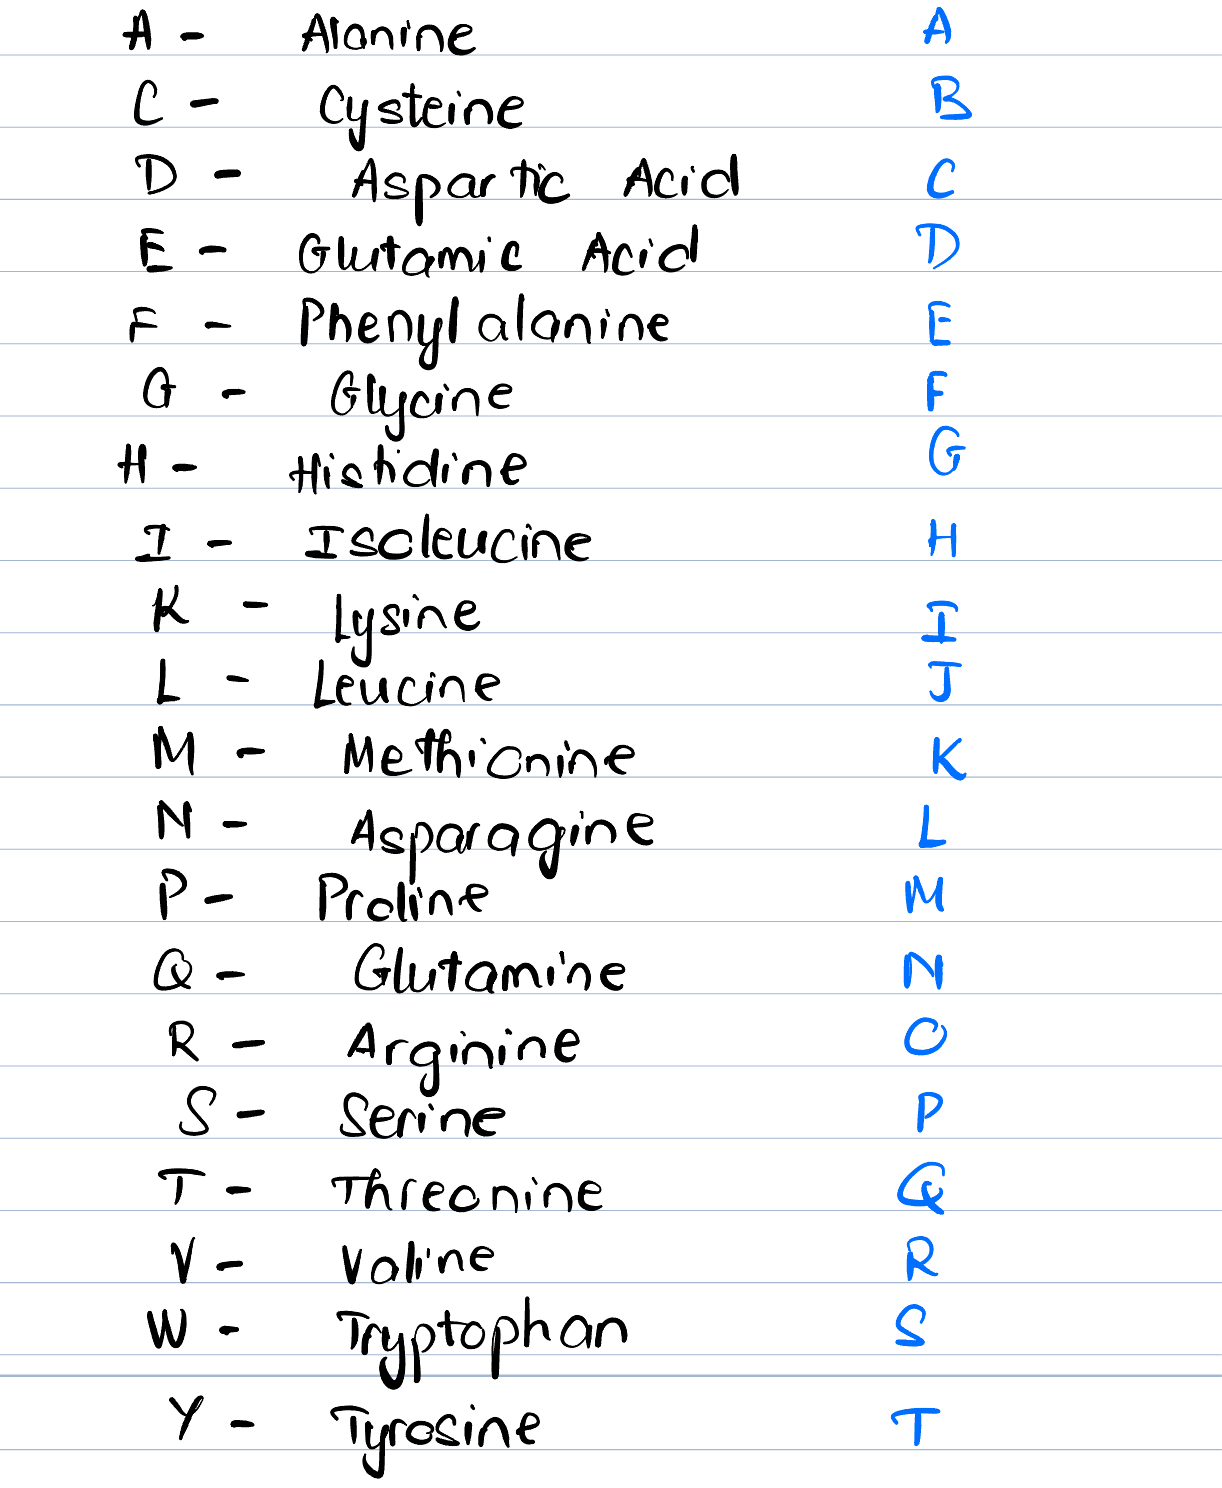
\includegraphics[width=\textwidth]{figures/Amino_Acid_Condensed_Form.jpg}
    \caption{List of Amino acids, the standard IUPAC single letter codes and our condensed character representation.}
    \label{fig:amino-acids}
\end{figure}


\noindent \textbf{\underline{SCP} :} A subset of the proteins, that occur only once in the genome, are termed as \textbf{single-copy proteins (SCPs)}. 
We use $\mathcal{P}_A$ to denote the set of SCPs in genome $G_A$.

\noindent \textbf{\underline{Tetramer} :} A \textbf{tetramer} is a substring of the protein and is of length 4. For example, the first three tetramers of the protein \texttt{MNRQGKSVEISELS} are  \texttt{MNRQ}, \texttt{NRQG} and \texttt{RQGK}.
For a protein $P_i$ and genome $G_A$, we denote $Q({P_i, G_A)}$ as the set of tetramers occurring in  $P_i$ of $G_A$.


\noindent \textbf{\underline{Average Jaccard Index} :} 
\textbf{Average Jaccard Index} of a pair of genomes A and genome B is defined as the following ratio :
\begin{equation}
    \label{eq:avgJaccard}
    AJI({G_A, G_B}) = \cfrac{
     \mathlarger{\sum_{ P_i \in \mathcal{P}_A \bigcap \mathcal{P}_B }}J({P_i, G_A, G_B})}{
     \mid \mathcal{P}_A \bigcap \mathcal{P}_B\mid}
\end{equation}
where $J({P_i, G_A, G_B})$ is defined as:
\begin{equation}
    \label{eq:pairwiseproteinJaccard}
    J(P_i, G_A, G_B) = \cfrac{|Q(P_i, G_A) \bigcap Q(P_i, G_B)|}{
    |Q(P_i, G_A) \bigcup Q(P_i, G_B)| }
\end{equation}

Though $AJI({G_A, G_B})$ can be defined in a weighted manner,  in this document, we focus only on the \textbf{Average Jaccard Index}. 


\subsection{Problem} 
\begin{tabular}{|p{12cm}|}
\hline \\
Given a database of genomes, calculate the Jaccard similarity between all pairs of genomes as the sum of the \textbf{Average Jaccard Index} between each pair of genomes. \\
\\
\hline
\end{tabular}

\section{Data Structures}

\subsection{Tetramer Representation}

In the current implementation of AAI, the tetramers are represented using 32-bit integers constructed via a charcter-to-ASCII mapping. For example, tetramer "\texttt{AAAC}" is represented by the integer 65656567.

Since there are 20 amino acids, there are $20^4 = 160,000$ possible tetramers.
We propose to encode our tetramer by mapping tetramer to an integer in the range $[0, 20^4 - 1]$ i.e., $[0,159,999]$. 
Instead of standard IUPAC single letter codes, we use the uppercase English characters in the alphabetical order.
We map the amino acids to its "condensed" character form as the table shown in figure~\ref{fig:amino-acids}. 



\subsection{Current Implementation}
\label{data:current}
Current implementation of AAI uses the following two tables for  to represent the tetramer data generated from the database of the genomes.

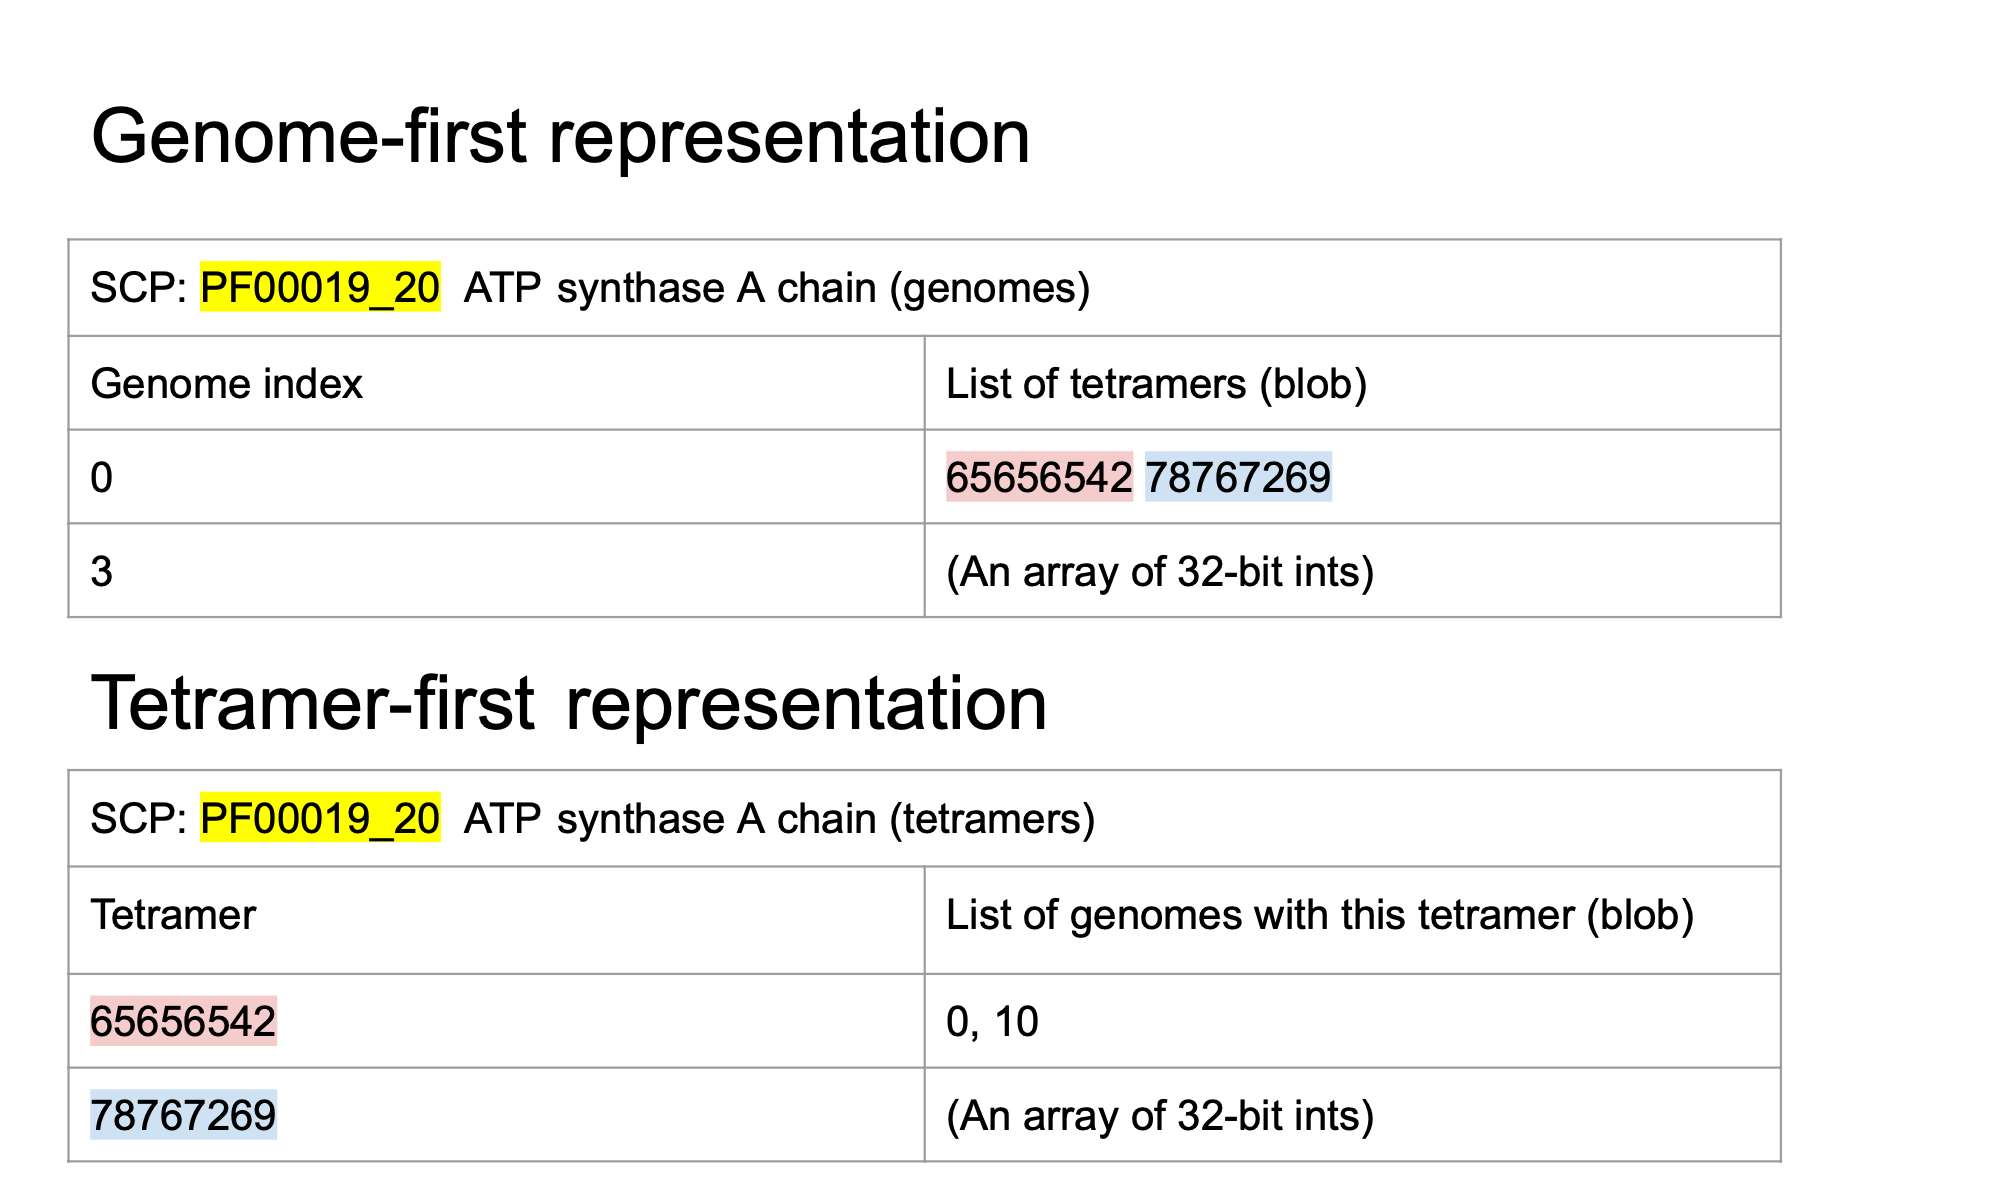
\includegraphics[width=\textwidth]{figures/Database_Representation.png}

For each single copy protein $P_i$, two tables are used : 
(i)  $DG_{P_i}$ Genome -- Tetramer table (which maps each genome to the list of tetramers stored in it), and
(ii) $DT_{P_i}$ Tetramer -- Genome table (which maps each tetramer to a list of genomes where this tetramer exists in). 


\subsection{Proposed Data Structures}
Let $\mathcal{G}$, $\mathcal{P}$ and  $\mathcal{T}$ be the set of all genomes, SCPs and tetramers present in the database respectively.
Correspondingly genomes, SCPs and tetramers are given identifiers in the ranges  $[0,|\mathcal{G}|-1]$, $[0,|\mathcal{P}|-1]$ and $[0,|\mathcal{T}|-1]$ respectively.  
Let $p$ be the number of processors available in the system. The processors are assigned identifiers in the range $[0,p-1]$. 

Our parallel algorithm uses the following four data structures. 
\begin{enumerate}
    \item $F$, a distributed array of protein, genome pairs, $(P_i, G_A)$. 
    For every tetramer $t_j, j\in\{0,\dots,20^4-1\}$, the array $F$ stores all pairs of $(P_i, G_A)$, if and only if the tetramer $t_j$ exists in SCP $P_i$ of Genome $G_A$. 
    $F$ stores this data as a blocks of sub-arrays for every $t_j$, in the ascending order of tetramers. 
    Within each block of information for a tetramer, the pairs are first sorted by the protein, and then by the genome. 
   
    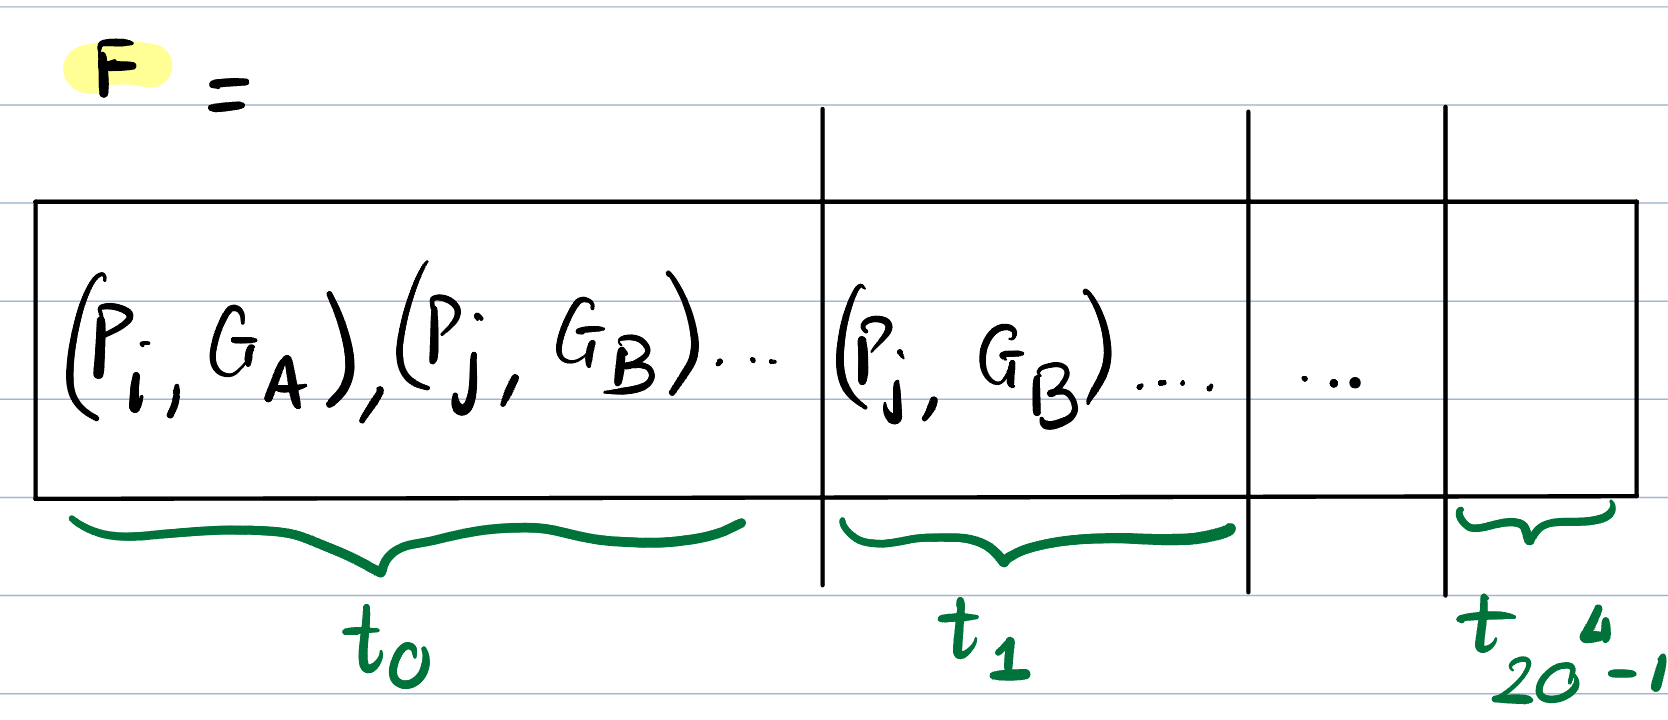
\includegraphics[width=\textwidth]{figures/F_table_tetramer_indexed.jpeg}
    
    \item $L_c$, an array of counts of length $20^4 = 160,000$, where $L_c[t_j]$ is size of the block corresponding to $t_j$. 
    In other words $L_c[t_j]$ contains the number of entries corresponding to $t_j$ in $F$.  
    
    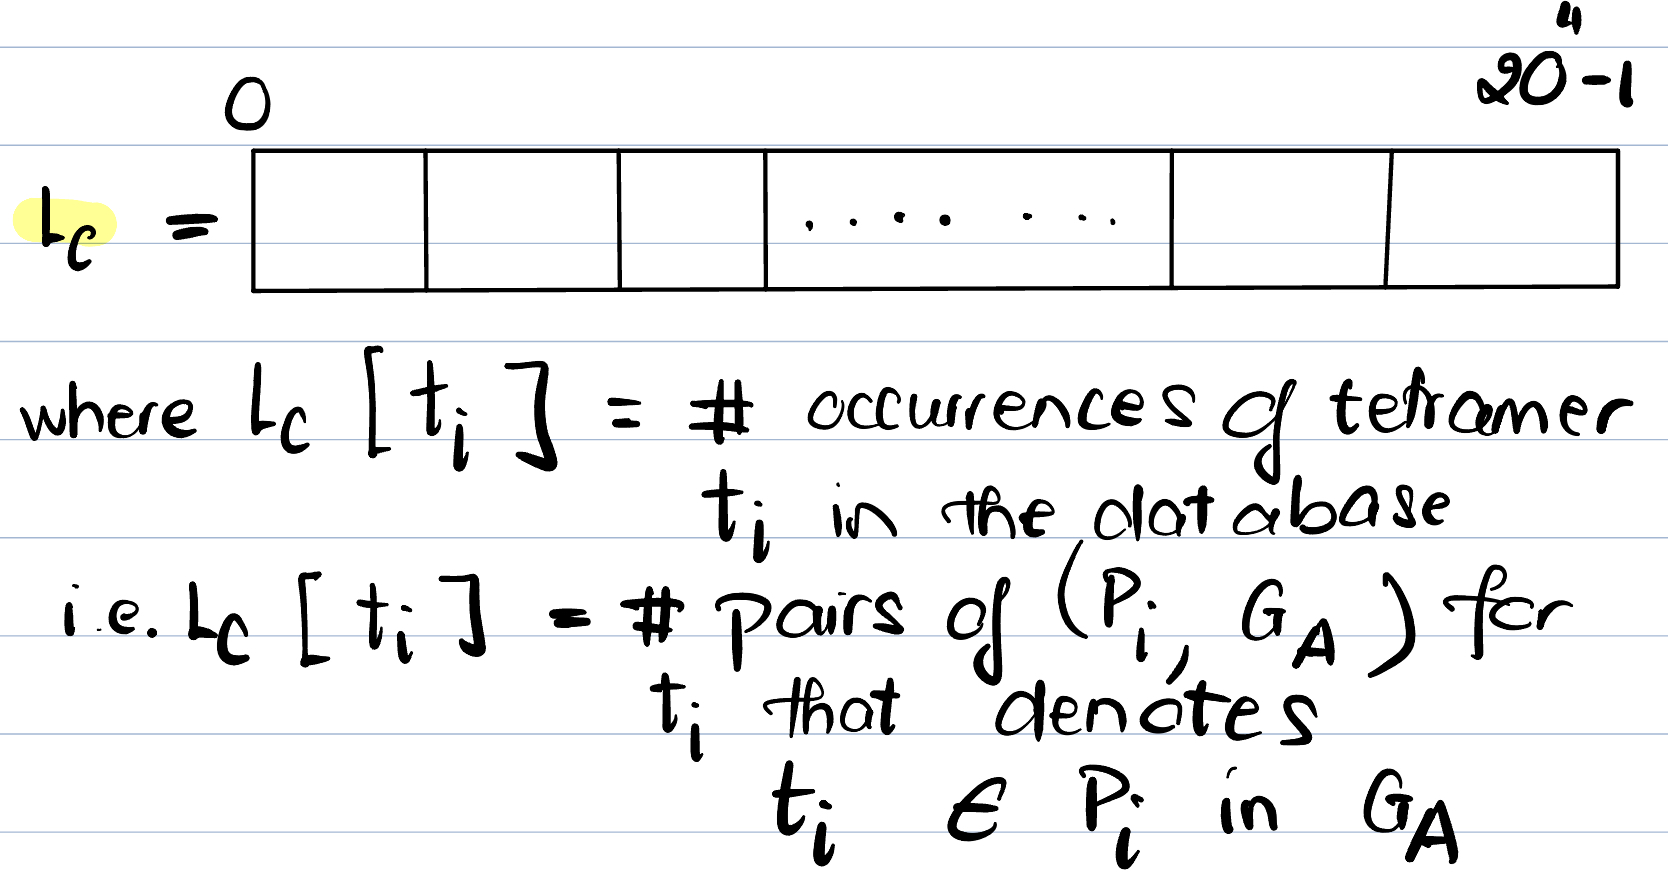
\includegraphics[width=\textwidth]{figures/Lc_table_tetramer_indexed.jpeg}

    \item $L_p$, a pointer array of length $20^4$.
    We construct the pointer array $L_p$ by performing a prefix sum on  $L_c$ i.e., $L_p[t_j] = \sum_{k < j} L_c[t_k]$.
    The array $L_p$ can be used to quickly identify the location of the block in $F$ corresponding to $t_j$ i.e., $L_p[t_j]$ locates the index of starting position corresponding to a the tetramer $t_j$ in of $F$ .
    
    
    \item $T$, a 2-D Array of size $|\mathcal{P}|\times|\mathcal{G}|$ that stores the number of tetramers in each of the SCP of every genome. 
    $T$ is required for computing the denominator of equation~\ref{eq:pairwiseproteinJaccard}.
    
    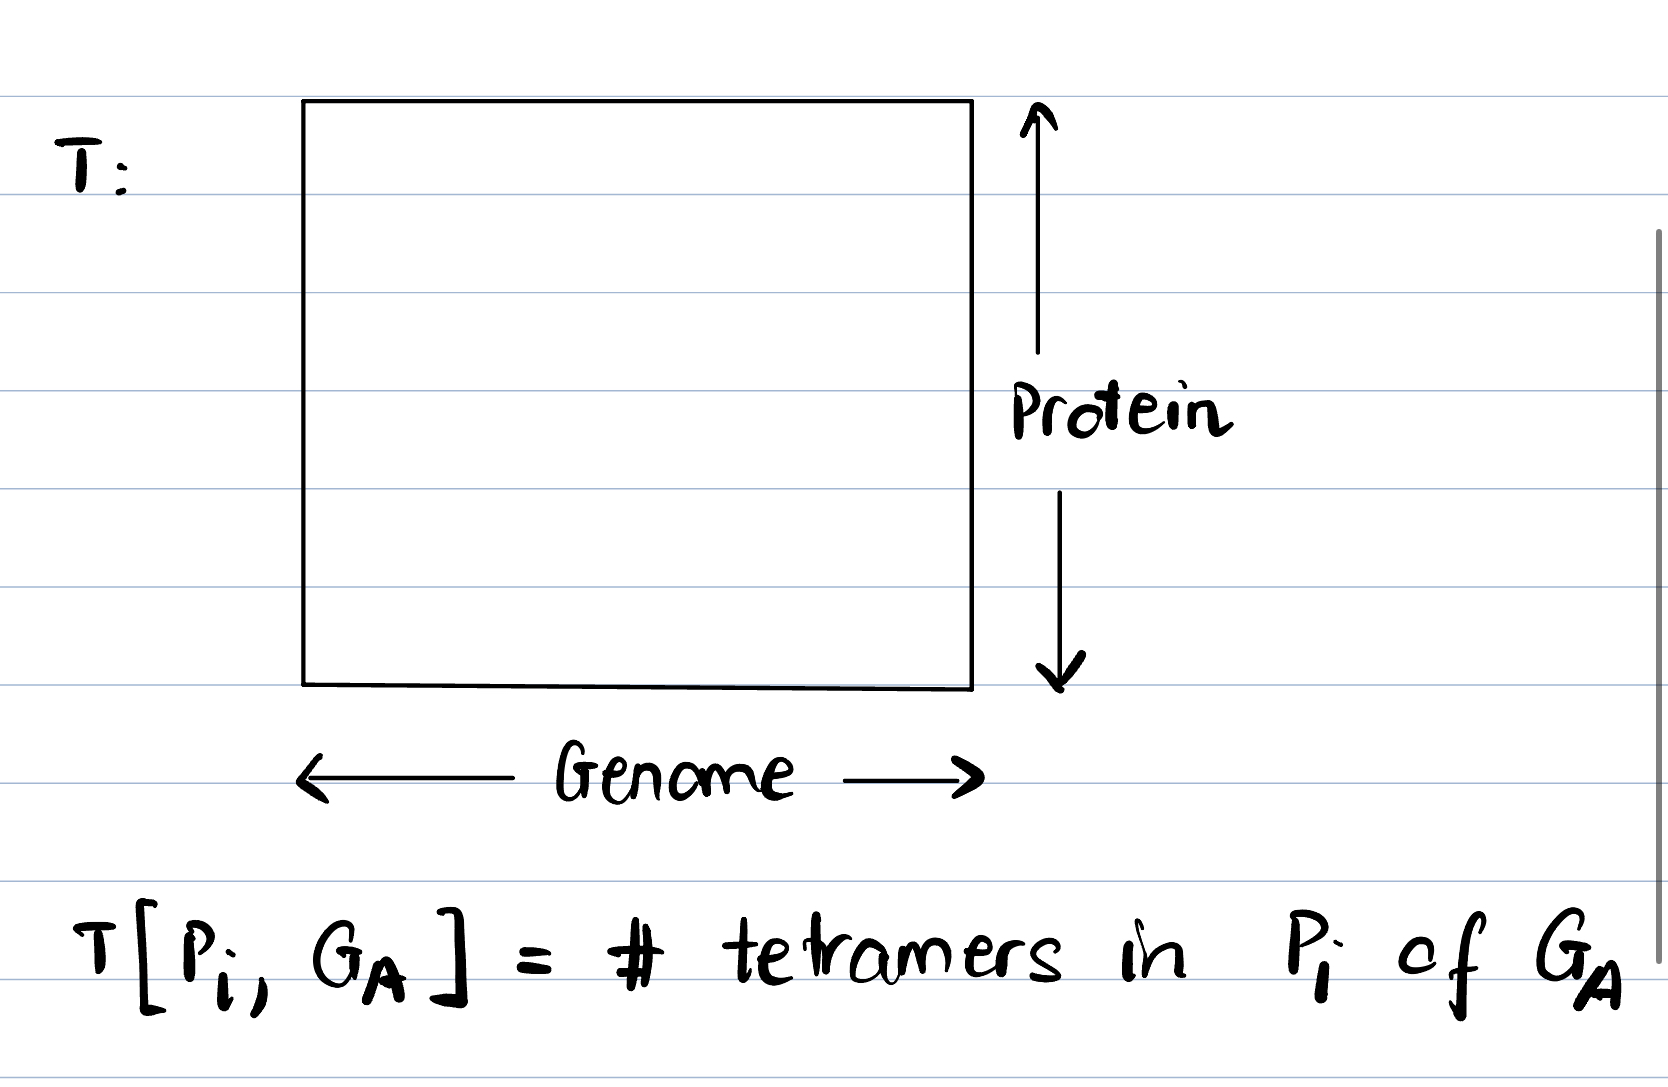
\includegraphics[width=\textwidth]{figures/T_table.jpeg}
    
    \underline{\textbf{Note}}: $|X \bigcup Y| = |X| + |Y| + |X \bigcap Y|$ for any 2 sets X and Y. The $T$ table stores the $|X|, |Y|$ values for our calculations. 
\end{enumerate}

\subsection{Construction of the proposed Data Structures}
We assume that the input datasets are available in memory in a format as shown in the section~\ref{data:current}.
The assumption implies that Tetramer--Genome tables ($DT$ tables) and Genome-Tetramer tables ($DG$ tables) are already constructed for the set of all SCPs, $\mathcal{P}$, as tables of pointers to arrays in memory. 
We also assume that enough memory is available to construct $F$, $L_c, L_p$ and $T$. 
If enough memory is not available to load all the proteins, the proteins can be processed in batches, with enough memory available to accommodate each batch. 
We further discuss this in section~\ref{sec:memoryconstraint}. 


We first construct the array $L_c$ array in parallel via algroithm~\ref{alg:constructLcTetramer} by counting the number of entries in $F$ corresponding to each tetramer across all proteins and genomes.
Each processor is assigned approximately $|\mathcal{T}|/p$ number of consecutive tetramers.
Algorithm~\ref{alg:constructFTetramer} enumerates the steps undertaken by processor with processor id $j$, to construct the part of the array corresponding to processor $j$, $L_{c,j}$. 
Since obtaining the total number of entries per protein is a constant operation, each processor executes $O((|\mathcal{T}| \times |\mathcal{P}|)/p)$ operations and hence, the algorithm takes $O((|\mathcal{T}| \times |\mathcal{P}|)/p)$ time. 

\begin{algorithm}[H]
\caption{Construct $L_c$ and $L_p$ in parallel}
\label{alg:constructLcTetramer}
\begin{algorithmic}[1]
\Function{Construct $L_c$ and $L_p$}{$\mathcal{P}$, $\mathcal{T}$,  $DT$, processor id $j$}
    \State [$t_{start}, t_{end}] \gets$ Tetramer range assigned to proc. $j$.
    \Comment  $\approx \cfrac{|\mathcal{T}|}{p}$ per proc.
    \State Initialize $L_{c,j}$ to zeros and  $|L_{c,j}| : t_{end} - t_{start} + 1$
    \Statex \; \; \; \textit{Note: $L_{c, j}$ the sub-array of $L_c$ corresponding to processor $j$}
    \For{each tetramer $t_k \in [t_{start}, t_{end}]$}
       \For{each protein $P_i \in \mathcal{P}$}
           \State $w$ $\gets$ Total no. of entries in $DT_{P_i}$ for tetramer $t_k$. 
           \State Increment $L_{c,j}[t_k - t_{start}]$ by $w$. 
       \EndFor
   \EndFor
   \State Construct $L_p$ as prefix sum $L_c$, i.e., $L_p[t_j] = \sum_{k < j} L_c[t_k]$
   \State \Return $L_c, L_p$
\EndFunction
\end{algorithmic}
\end{algorithm}


Algorithm~\ref{alg:constructFTetramer} presents our proposed parallel algorithm to construct $F$ in parallel.
Similar to Algorithm~\ref{alg:constructLcTetramer}, algorithm~\ref{alg:constructFTetramer} lists only the steps undertaken by processor $j$, to construct the block of the array $F$ corresponding to processor $j$. We denote this block as $F_j$. 

The algorithm assigns a range of tetramers to each processor based on the number entries in $F$ corresponding the those tetrarmers. 
The tetramers are distributed such that each processor constructs approximately $|F|/p$ number of entries in $F$. 
In order to identify the size of the $F$ block that corresponds to a range of tetramers, the algorithm makes use of the $L_c$ array.

After the assignment, the relevant data is queried from the relevant $DT$ tables, and then, the algorithm proceeds to append entries to $F_j$ portion of $F$ and update $L_{c,j}$ whenever $F_j$ is extended.

\begin{algorithm}[H]
\caption{Construct $F$ in parallel}
\label{alg:constructFTetramer}
\begin{algorithmic}[1]
\Function{Construct $F$}{$\mathcal{P}$, $\mathcal{T}$,  $DT$, processor id $j$}
    \State [$t_{start}, t_{end}] \gets$ Tetramer range w.r.t proc. $j$. from $L_p$
    \Statex \; \; \; \textit{Note: Tetramers are distributed such that each processor constructs approximately $|F|/p$ number of entries in $F$}
    \State $F\gets$ Distributed array of (protein, genome) pairs
    \Comment  $\approx \cfrac{|F|}{p}$ per proc.
    % \Statex \; \; \; $F_{j}\gets$ Initialize $t_{e} - t_{s} + 1$ entries of (protein, genome) pairs.
    \Statex \; \; \; \textit{Note: $F_j$ the sub-array of $F$ corresponding to processor $j$}
    \For{each tetramer $t_k \in [t_{start}, t_{end}]$}
      \For{each protein $P_l \in \mathcal{P}$}
           \State $SDT$ $\gets$ Query in $DT_p$ for tetramer $t_k$. 
           \State Sort $SDT[t_k]$ by genome ids, if needed.
           \For{each genome $G_A$ in $SDT[t_l]$}
               \State Append $(P_l, G_A)$ to $F_j[t_k]$.
           \EndFor
        \EndFor
   \EndFor
\EndFunction
\end{algorithmic}
\end{algorithm}
Since the entries of $F$ are distributed approximately equally across the $p$ processors, this algorithm takes $O(|F|/p)$ time.

Algorithm~\ref{alg:constructTTetramer} depicts our proposed algorithm to build the two dimensional array $T$ of size $|\mathcal{P}| \times |\mathcal{G}|$. 
In parallel construction of $T$, the rows are distributed equally across each processor.
Each processor constructs a slice of $T$, as sub-matrix of size $\frac{|\mathcal{P}|}{p} \times |\mathcal{G}|$.
The locally compute $T$ is then broadcast to all the other processors, after which, each processor gets access to $T$ in its entirety. 
\begin{algorithm}[H]
\caption{Construct $T$ in parallel}
\label{alg:constructTTetramer}
    \begin{algorithmic}[1]
        \Function{Construct $T$}{$\mathcal{P}$, $\mathcal{T}$, $DG$, processor id $j$ }:
          %\State Assign $\approx \cfrac{\mathcal{P}}{n_p}$ per processor.
          \State $P_{start}, P_{end} \gets$ Proteins assigned to proc. j
          \Comment  $\approx \cfrac{|\mathcal{P}|}{p}$ per proc.
          \State $T\gets$ Initialize 2D array of size $|\mathcal{P}|\times |\mathcal{G}|$
          \For{protein $P_k \in [P_{start}, P_{end}]$} 
             \State $SDG \gets$ Query $DG_{P_k}$.
             \For{genome $G_l \in SDG$}
                    \State $T[P_k, G_l] \gets|SDG[G_l]| - 3$
             \EndFor
          \EndFor
          \State Broadcast locally-computed $T$ to all the processors.
        \EndFunction
    \end{algorithmic}
\end{algorithm}
Since size of the $T$ is relatively small compared to $F$, this is expected to consume much less time compare to the construction of $F$ and the algorithm to compute Average Jaccard Index.

\subsection{Handling Memory Constraints}
\label{sec:memoryconstraint}
In case of running the algorithm in a old desktop or laptop with limited main memory, all the protein and tetramer data may not be completely loaded in the main memory.
In such cases, the above algorithms can be run in batches of protein.
In each batch, only a subset of SCPs are processed at a time. 
Here, $F$ and $L_c$ will be rebuilt while processing each batch, where as $T$ will be constructed only once and retained in the main memory. 


\section{Parallel FastAAI Algorithm}

%         Calculate the \textbf{batches of protein bp} (where to start, where to end in each batch)
Algorithm~\ref{alg:fastAAIParallelTetramer} enumerates the key steps our parallel algorithm for FastAAI as executed by processor $j$. After constructing the data structures in lines \ref{constructBeginTetramer} -- \ref{constructEndTetramer}, the algorithm proceeds to construct a distributed array $E$, containing the tuples $(P_i, G_A, G_B)$ for each tetramer matched in protein $P_i$ between $G_A$ and $G_B$ (lines~\ref{ebeginTetramer}-~\ref{eendTetramer}).

Sorting the array $E$ by genome pairs brings the entries corresponding to the same genome pairs can be processed together to compute the Jaccard coefficients. We accomplish this in lines~\ref{jacbeginTetramer} --~\ref{jacendTetramer} using the distributed array $JAC$ of tuples $((G_A, G_B), S, N)$, where $S$ and $N$ maintain the sum of Jaccard coefficients and number of common proteins respectively.

After eliminating the duplicates in $JAC$ array, the AJI values can be computed with a scan across the $JAC$ array (lines \ref{ajibeginTetramer}--\ref{ajiendTetramer}).

Each step in the algorithm distributes the work equally among all the processors, the algorithm is efficiently parallel.
\begin{algorithm}[H]
\caption{FastAAI Parallel Algorithm}
\label{alg:fastAAIParallelTetramer}
\begin{algorithmic}[1]
    \Function{Parallel fastAAI}{$\mathcal{P}$, $\mathcal{T}$, $DT$, $DG$, processor $j$}:
        % TODO: \State $(G_A, G_B)_{start}, (G_A, G_B)_{end} \gets$ Range of Genome pairs for proc. $j$.
        %\Comment $\approx \frac{\binom{|\mathcal{G}|}{2}}{p}$ per proc.
        \Statex \underline{Phase 1 : Construction of the data structures}
        \State \label{constructBeginTetramer} $L_c, L_p \gets$ \Call{Construct $L_c$}{$\mathcal{P}$, $\mathcal{T}$,  $DT$, processor id $j$}
        \State $F \gets $ \Call{Construct $F$}{$\mathcal{P}$, $\mathcal{T}$,  $DT$, processor id $j$}
        \State \label{constructEndTetramer}  $T \gets $ \Call{Construct $T$}{$\mathcal{P}$, $\mathcal{T}$, $DG$, processor id $j$ }
        \Statex \underline{Phase 2 : Generate tetramer tuples}
        \State $[t_{start}, t_{end}] \gets$ Tetramers assigned to proc. $j$ using $L_p$.
        % \Comment  $\approx \cfrac{|F|}{n_p}$ per proc.
        \Statex \; \; \; \textit{Note: Tetramers are distributed s.t. a processor is assigned  $\approx |F|/p$ entries.}
        \State \label{ebeginTetramer} $E : $ Distributed array of tuples $(P_i, G_A, G_B)$.
        \Statex \; \; \; \textit{Note: $E_j$ is the sub-array corresponding to processor $j$.}
        \For{each tetramer $t_k \in [t_{start}, t_{end}]$}
           \For{each block $B_l$ in $F_j$ w.r.t. protein $P_i$, and tetramer $t_k$ }
              \For{each pair $(G_A,G_B)$ in block $B_l$}
                  \State Append the tuple $(P_i, G_A, G_B)$ to $E_j$
              \EndFor
           \EndFor
        \EndFor
        \State \label{eendTetramer} Parallel sort $E$ by $(G_A, G_B)$, and then by $P_i$. 
        \Statex \underline{Phase 3 : Compute the Jaccard Coefficient values} 
        \State \label{jacbeginTetramer} $JAC :$  Distributed array  of tuples $((G_A, G_B), S, N)$, where 
        \Statex \; \; \; \; - $(G_A, G_B)$ is a genome pair, 
        \Statex \; \; \; \; - $S$ is $\sum_i J(P_i, G_A, G_B)$ w.r.t. the tuples in $F$ processed so far, and
        \Statex \; \; \; \; - $N$ is $|\mathcal{P}_A \cap \mathcal{P}_B|$ w.r.t the tuples in $F$ processed so far.
        \Statex \; \; \; \; \textit{Note: $JAC_j$ is the sub-array corresponding to processor $j$.}
        % $|RST_{j}| : $ No. of gene pairs assigned to proc. $j$
        %[\verb|#|genome in range [$(G_A, G_B)_{start}, (G_A, G_B)_{end}$]]
        %\State Send subarrays of E made up of the same $G_A, G_B$ to the processor responsible for the pair. 
        \For{each block $B_l$ of $E_j$ with the same genome pair $(G_A, G_B)$}
            \State $S \gets 0$; $N \gets 0$
               \For{each sub-block $B_k$ of $B_l$ with the same protein $P_i$}
                  %\State $\gamma \gets |B_l|$
                   \State $J_{P_i, G_A, G_B}\gets\cfrac{|B_k|}{T[P_i, G_A] + T[P_i, G_B] - |B_k|}$
                   \State Increment $S$ by $J_{P_i, G_A, G_B}$.
                   \State Increment $N$ by 1.
                   %\State output[$G_A, G_B$][1] += 1
                   %\TODO: If{$\gamma > 0$}
                   %\EndIf
            \EndFor
            \State Append $((G_A, G_B), S, N)$ to the table $JAC_j$ 
        \EndFor
        \State \label{jacendTetramer} Remove the duplicate entries in $JAC$ for a given $(G_A, G_B)$ pair by summing up the corresponding $S$ and $N$ values.
        \State \label{ajibeginTetramer} $AJI :$ Map of AJI values.
        \For{each entry of $((G_A, G_B), S, N) \in JAC_j$  }
            \State $AJI[(G_A, G_B)] = \cfrac{S}{N}$
        \EndFor \label{ajiendTetramer}
    \EndFunction
\end{algorithmic}
\end{algorithm}


%        \begin{enumerate}
%            \item \textbf{for proteinBatch} in bp:
%            \begin{enumerate}
%                \item F, $L_c \gets$ constructFTetramerandLc(database, proteinBatch, $tet_{start}, tet_{end}$)
%                \item E$\gets$ empty vector
%                \item \textbf{for tetramer t} in $[tet_{start}, tet_{end}]$:
%                \begin{enumerate}
%                    \item[] \textbf{for block of same protein $P_i$} in F[t]:
%                    \begin{enumerate}
%                        \item[] \textbf{for all pairs $G_A, G_B$} in \textbf{block}:
%                        \begin{itemize}
%                            \item[] E.append(($P_i, G_A, G_B$))
%                        \end{itemize}
%                    \end{enumerate}
%                \end{enumerate}
%                \item Parallel sort E by $G_A, G_B$, and then by p. 
%                \item Send subarrays of E made up of the same $G_A, G_B$ to the processor responsible for the pair. 
%                \item \textbf{for block of the same $G_A, G_B, P_i$} in E:
%                \begin{itemize}
%                    \item[] $\gamma\gets$ length of block
%                    \item[] $J_{P_i, G_A, G_B}\gets\cfrac{\gamma}{T[P_i, G_A] + T[P_i, G_B] - \gamma}$
%                    \item[] output[$G_A, G_B$][0] += $J_{P_i, G_A, G_B}$
%                    \item[] if $\gamma > 0$:
%                    \begin{itemize}
%                        \item[] output[$G_A, G_B$][1] += 1
%                    \end{itemize}
%                \end{itemize}
%                \item \textbf{for all pairs of $G_A, G_B$} in [$(G_A, G_B)_{start}, (G_A, G_B)_{end}$]:
%                \begin{itemize}
%                    \item[] result[$G_A, G_B$] = $\cfrac{output[G_A, G_B][0]}{output[G_A, G_B][1]}$
%                \end{itemize}
%            \end{enumerate}
%        \end{enumerate}
%
\end{document}

